\documentclass[8pt]{beamer}

\newif\ifplacelogo % create a new conditional
\placelogotrue % set it to true

\usetheme{Warsaw}
\usecolortheme{rose}
\usepackage{multicol}
\usepackage{epstopdf}
\usepackage[italic]{hepnames}
\usepackage{tikz}
\usepackage{listings}
\usepackage{times}
\usepackage{amsmath}
\usepackage{verbatim}
\usepackage{hyperref}
\usepackage{bbding}
\lstset{breakatwhitespace,
language=C++,
columns=fullflexible,
keepspaces,
breaklines,
tabsize=3, 
showstringspaces=false,
extendedchars=true}

% TikZ includes!!!
\usepackage{tikz}
\usetikzlibrary{backgrounds}
\usetikzlibrary{calc}
\tikzstyle{every picture}+=[remember picture]
\input{/home/oviazlo/Desktop/beamerPresentations/myReports/latexHelpScripts/tikzGrid.tex}


\begin{document}

% custom colors
\definecolor{olive}{rgb}{0.3, 0.4, .1}
\definecolor{fore}{RGB}{249,242,215}
\definecolor{back}{RGB}{51,51,51}
\definecolor{title}{RGB}{255,0,90}
\definecolor{dgreen}{rgb}{0.,0.6,0.}
\definecolor{gold}{rgb}{1.,0.84,0.}
\definecolor{JungleGreen}{cmyk}{0.99,0,0.52,0}
\definecolor{BlueGreen}{cmyk}{0.85,0,0.33,0}
\definecolor{RawSienna}{cmyk}{0,0.72,1,0.45}
\definecolor{Magenta}{cmyk}{0,1,0,0}

\definecolor{PixelColor}{RGB}{207,232,139}
\definecolor{SCTColor}{RGB}{167,166,255}
\definecolor{TRTColor}{RGB}{250,224,140}
\definecolor{grayColor}{RGB}{153,153,153}

\newcommand{\yRefPosOne}{0.0}
\newcommand{\xRefPosOne}{0.0}
\newcommand{\yRefPosTwo}{0.0}
\newcommand{\xRefPosTwo}{0.0}
\newcommand{\yRefIncrementOne}{0.0}
\newcommand{\xRefIncrementOne}{0.0}
\newcommand{\yRefIncrementTwo}{0.0}
\newcommand{\xRefIncrementTwo}{0.0}

\graphicspath{ {/home/oviazlo/Desktop/beamerPresentations/FCCee/pictures/plots_CALICE_workshop/} }


\DeclareGraphicsExtensions{.eps, .pdf, .png}

\newcommand{\myBox}[2][pink] {
    \noindent\colorbox{#1}{
	\textbf{#2}
    }\par
}

% For nice block (provided by Oleh)
\tikzstyle{myBox} = [draw=red, fill=blue!1, very thick,
    rectangle, rounded corners, inner sep=5pt, inner ysep=9pt]
    
\tikzstyle{PixelBox} = [draw=PixelColor, fill=blue!1, very thick,
    rectangle, rounded corners, inner sep=5pt, inner ysep=9pt]
\tikzstyle{SCTBox} = [draw=SCTColor, fill=blue!1, very thick,
    rectangle, rounded corners, inner sep=5pt, inner ysep=9pt]
\tikzstyle{TRTBox} = [draw=TRTColor, fill=blue!1, very thick,
    rectangle, rounded corners, inner sep=5pt, inner ysep=9pt]

% poster advertisement
\newcommand{\myCenterBox}[2][pink] {
   {\centering
    \noindent\colorbox{#1}{
	\textbf{#2}
    }\par
  }
}

\newcommand{\mySmallCenterBox}[2][pink] {
   {\centering
    \noindent\colorbox{#1}{
	\textbf{{\small #2}}
    }\par
  }
}

\newcommand{\myVerySmallCenterBox}[2][pink] {
   {\centering
    \noindent\colorbox{#1}{
	\textbf{{\scriptsize #2}}
    }\par
  }
}

\newcommand{\backupbegin}{
   \newcounter{finalframe}
   \setcounter{finalframe}{\value{framenumber}}
}
\newcommand{\backupend}{
   \setcounter{framenumber}{\value{finalframe}}
}

\newcommand{\myNode}{\tikz[baseline,inner sep=1pt] \node[anchor=base]}

\tikzstyle{fancytitle} =[fill=white!15, text=black]

\definecolor{light-gray}{gray}{0.95}
% poster advertisement


\title[ ??? \hspace{13.5em}\insertframenumber/
\inserttotalframenumber]{ ??? }


	\author[Oleksandr Viazlo, Matthias Weber]{Oleksandr Viazlo, Matthias Weber \\ 
% 	{\small ???}
	}
	\institute{\small CERN\\} 
	
       
	\date{9 March 2018}

% 	\logo{ \ifplacelogo \includegraphics[height=1.8cm]{./ID_week2/lund_uni-logo_s.pdf} \hspace{0.4cm} \fi}

	
   	\frame{\titlepage}

   	

\placelogofalse

%------------------------------------------------
\begin{frame}
\frametitle{Introduction} 

\renewcommand{\yRefPosOne}{0}
\renewcommand{\xRefPosOne}{5.3}
\renewcommand{\xRefIncrementOne}{5.5}

\begin{tikzpicture}[overlay]

\node [myBox, anchor=north west] at (-0.5,3) (box){%
    \begin{minipage}{0.45\textwidth}
        \begin{itemize}
         \item Compact Linear Collider
         \item 3 energy stages: \\ 380  GeV, 1.5 TeV, 3 TeV
         \item ??? Bunch trains separated with 20 $\mu$$m$
        \end{itemize}
    \end{minipage}
};
\node[fancytitle, right=15pt] at (box.north west) {CLIC};

\node [myBox, anchor=north east] at (11.0,3) (box){%
    \begin{minipage}{0.45\textwidth}
        \begin{itemize}
         \item Future Circular Collider ($e^-e^+$)
         \item 4 energy stages: $Z$, $WW$, $HZ$, $t\bar{t}$
         \item Bunch spacing: 20 - 8533 ns
        \end{itemize}
    \end{minipage}
};
\node[fancytitle, right=15pt] at (box.north west) {FCC-ee};

% \node [myBox, anchor=north east] at (11.0,-1) (box){%
\node [anchor=north east] at (12,0) (box){%
    \begin{minipage}{0.5\textwidth}
        \begin{itemize}
         \item Both experiments demands state-of-the-art detectors with:
         \begin{itemize}
          \item low-material tracking system
          \item high-granularity calorimeters
         \end{itemize}
        \hspace{0.2cm} \\
         \item CLICdet - proposed detector model \\ for CLIC with 4 Tesla magnetic field \\
         \hspace{0.2cm} \\
         \item CLD - detector model for FCC-ee derived from CLICdet and optimized for FCC-ee experimental conditions \\ (e.g. 2 Tesla magnetic field)
        \end{itemize}
    \end{minipage}
};
% \node[fancytitle, right=15pt] at (box.north west) {Search for $\PWprime$};

 
  \node[inner sep=0pt] (tmp) at (\xRefPosOne-2.35,\yRefPosOne-2.3)
    {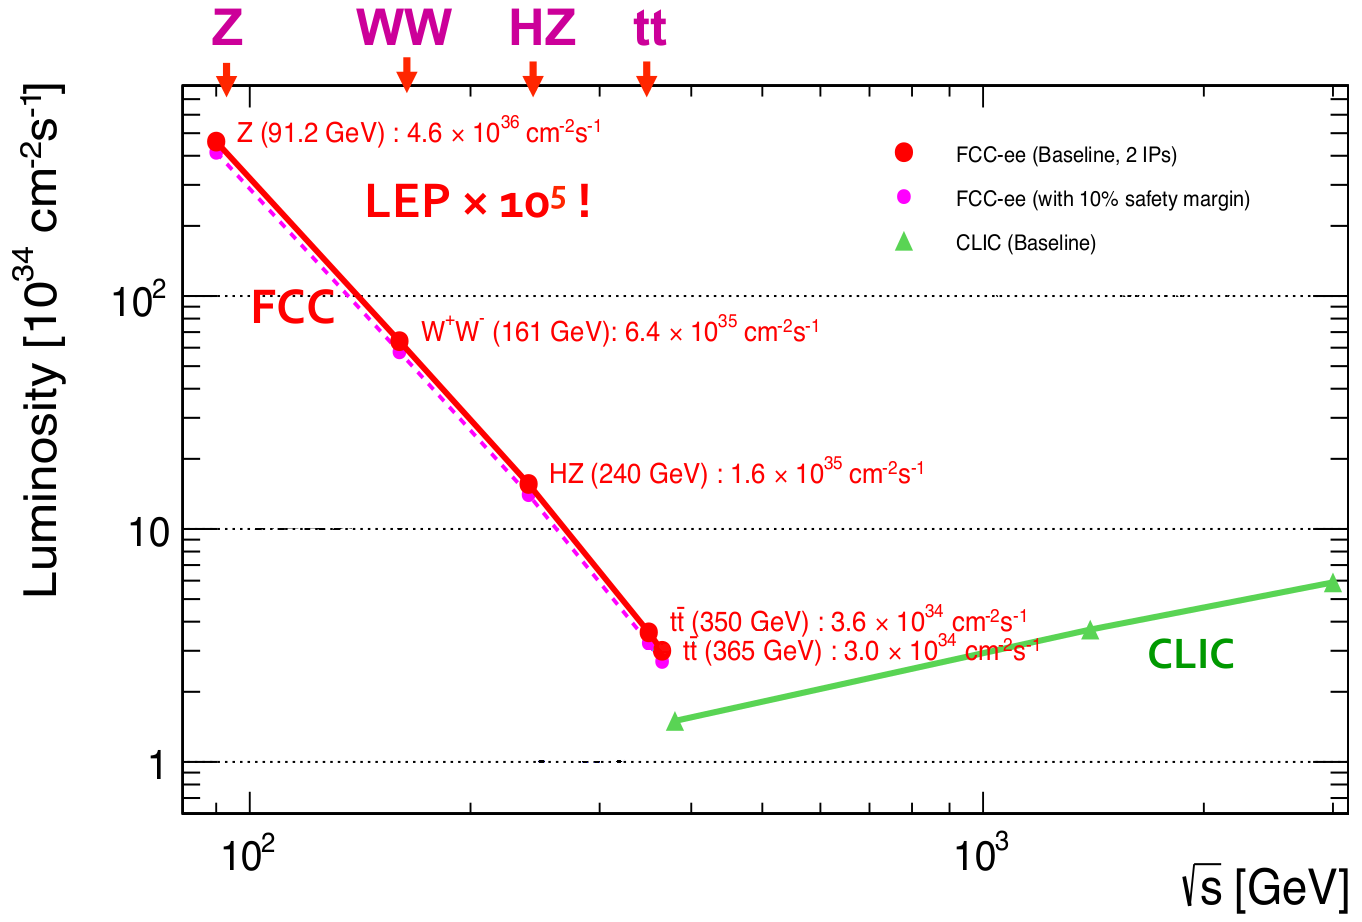
\includegraphics[width=7.5cm]{../CEPC_workshop/FCCee_lumi_vs_others_v2.png}};
 
%% HELPER draw advanced helping grid with axises:
% \draw(-0.5,-4) to[grid with coordinates] (11.5,4);

\end{tikzpicture}
\end{frame}
%------------------------------------------------


%*****************************************************************************
\begin{frame}{\large \large CLD and CLICdet detector models}

\renewcommand{\yRefPosOne}{0}
\renewcommand{\xRefPosOne}{5.3}
\renewcommand{\xRefIncrementOne}{5.5}
\begin{tikzpicture}[overlay]

 \node[inner sep=0pt] (tmp) at (\xRefPosOne-2.15,\yRefPosOne-0.56)
    {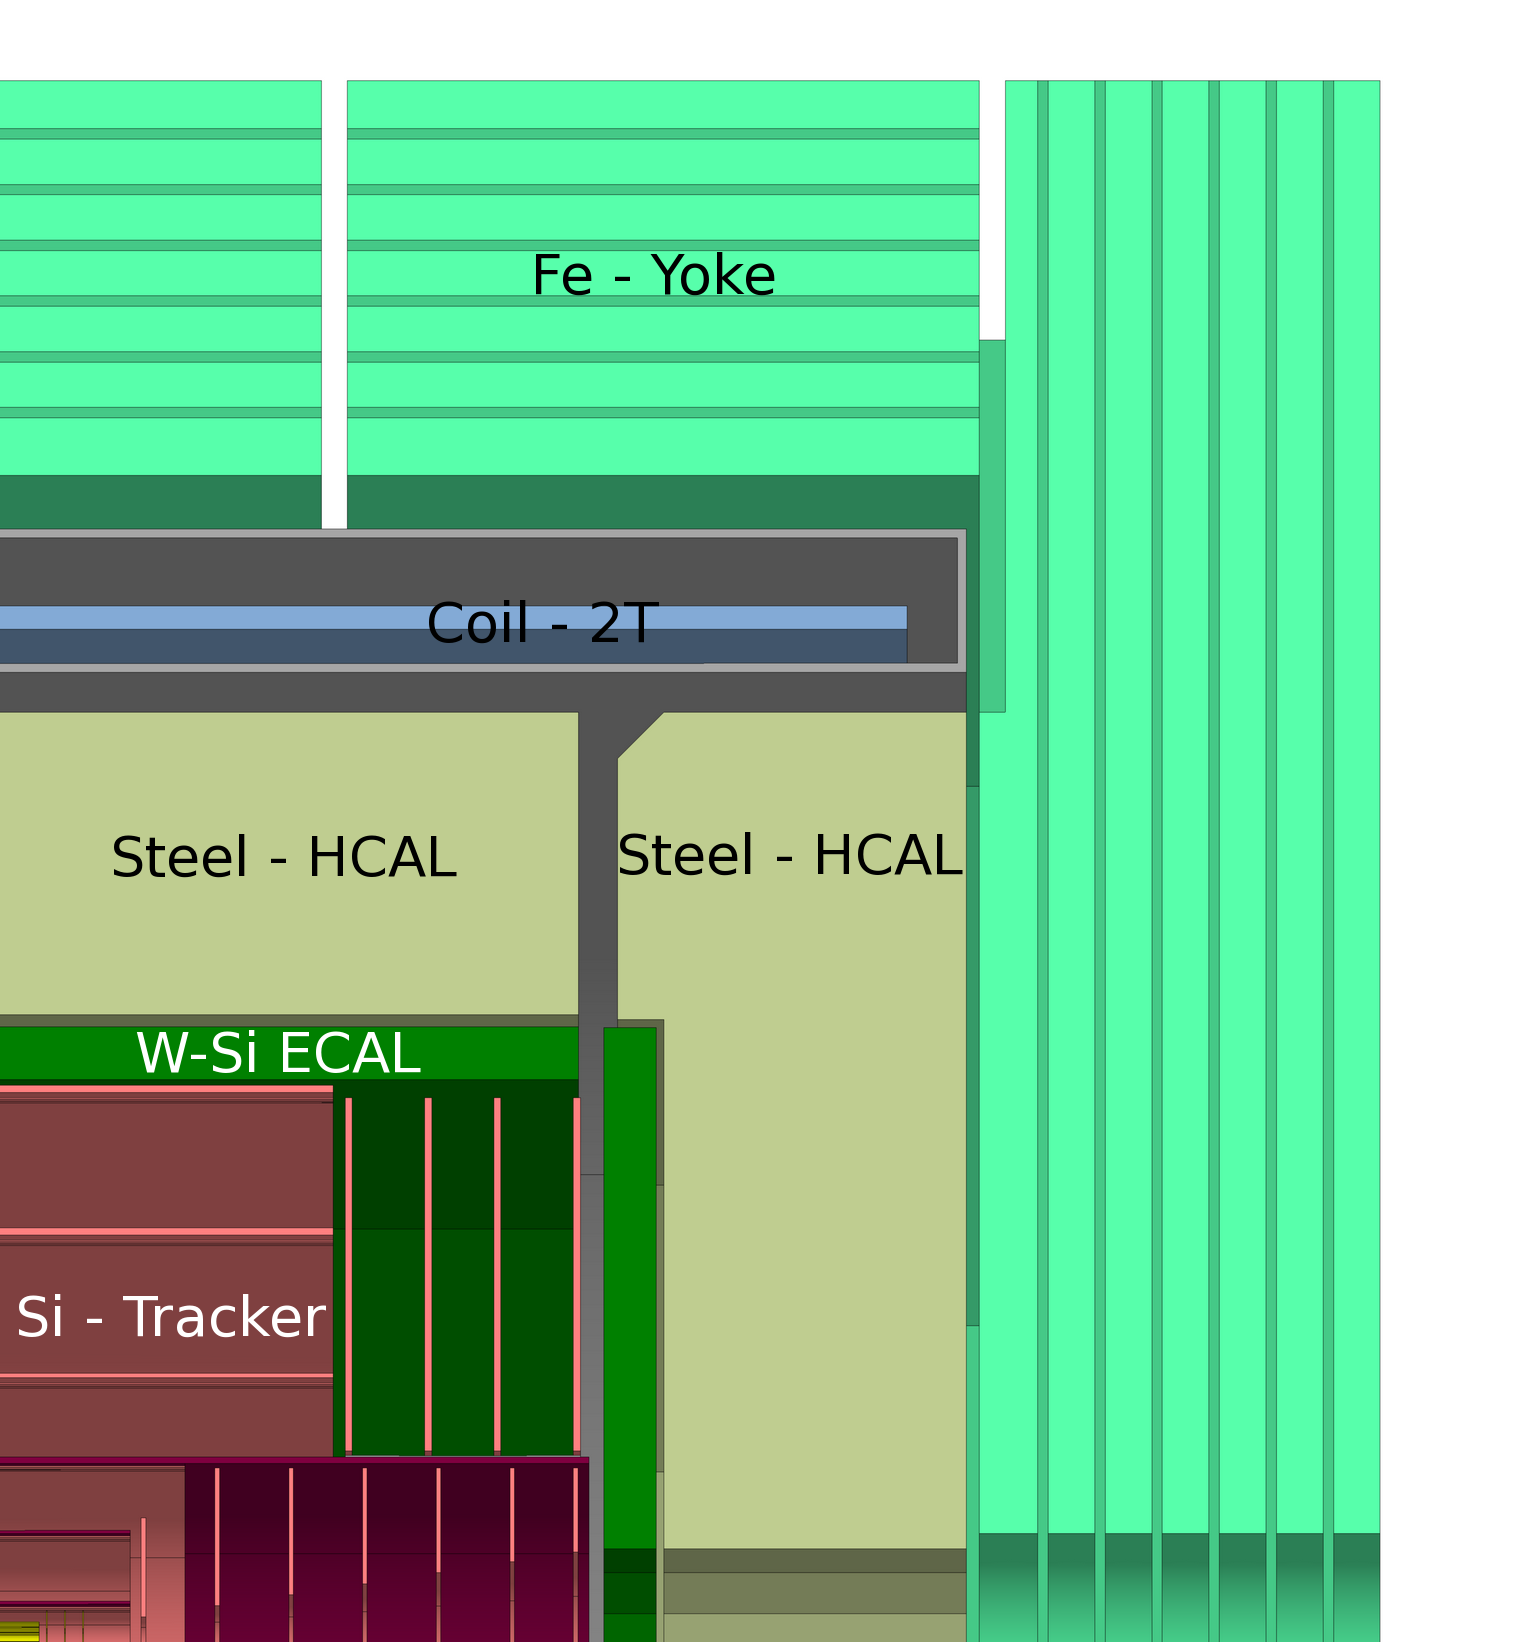
\includegraphics[width=7.8cm]{../CEPC_workshop/FCCeePictsFromKonrad/CLIC_FCC_Top_QuarterView_withLabes.png}};

\node  at (\xRefPosOne,\yRefPosOne+2.8) (box){%
\myCenterBox{\small CLD model}
}; 
    
    \draw[black, thick, ->] (-0.8,-4.76)--(-0.8,3.7) node[pos=0.95, right]{\small R [m]};
    \draw[black, thick, ->] (-0.8,-4.76)--(6.5,-4.76) node[pos=0.95, below]{\tiny Z [m]};
    
  \node[inner sep=0pt] (tmp) at (\xRefPosOne-3.05,\yRefPosOne-4.9)
    {2.3};   
  \node[inner sep=0pt] (tmp) at (\xRefPosOne-1.14,\yRefPosOne-4.9)
    {3.7};  
    
%     \node [PixelBox] at (\xRefPosOne+3.7,\yRefPosOne-4) (box){%
%   \begin{minipage}{0.43\textwidth}
%     Detector design inspired by detectors for CLIC and ILC and optimized for FCC-ee conditions
%   \end{minipage}
% };

\node  at (\xRefPosOne+3.5,\yRefPosOne-0.5) (box){%
    \begin{minipage}{0.5\textwidth}

  \begin{itemize}
      \item 4 Tesla magnetic field \\
   {\color{red} 2 Tesla magnetic field - CLD} \\ [0.3cm]
   \item Full silicon VTX and Tracker:  
   \begin{itemize}
   
    \item $\geqslant$12 hits per track 
    \item r$_{inner} = 31$mm, r$_{outer} = 1.5$m   \\
         {\color{red} r$_{inner} = 17$mm, r$_{outer} = 2.1$m - CLD}\\[0.3cm]
    
   \end{itemize}

   
%    \\ \hspace{0.1cm}  r$_{inner} = 17$mm, r$_{outer} = 2.1$m \\ \hspace{0.1cm} $\geqslant$12 hits per track
   \item W-Si ECAL 
   \begin{itemize}
    \item 40 layers, 22 X$_0$ \\[0.3cm]
   \end{itemize}
   \item Fe-Scint HCAL
   \begin{itemize}
    \item 60 layers, 7.0 $\lambda_I$ \\
    {\color{red}  44 layers, 5.5 $\lambda_I$ - CLD}\\
    [0.3cm] 
   \end{itemize}
%    Coil is outside of the calorimeter\\
   \item Steel return yoke with 6 RPC muon chambers: 
   \begin{itemize}
    \item 2 m thickness \\
    {\color{red}  1.5 m thickness - CLD}  \\[0.3cm]
   \end{itemize}

   
   
   \item CLICdet provide larger coverage of forward region \\
   {\color{red}   CLD - MDI (forward region): $<$ 150 mrad, 
   accommodates LumiCal }\\[0.3cm]
  \end{itemize}

    \end{minipage}
};


% \node [PixelBox] at (\xRefPosOne+3.7,\yRefPosOne-4) (box){%
%   \begin{minipage}{0.43\textwidth}
%     Detector design inspired by detectors for CLIC and ILC and optimized for FCC-ee conditions
%   \end{minipage}
% };

%% HELPER draw advanced helping grid with axises:
% \draw(-0.5,-4) to[grid with coordinates] (11.5,4);
\end{tikzpicture}

 
\end{frame}
%*****************************************************************************



%*****************************************************************************
\begin{frame}{\large \large CLD and CLICdet detector models}

\renewcommand{\yRefPosOne}{0}
\renewcommand{\xRefPosOne}{5.3}
\renewcommand{\xRefIncrementOne}{5.5}
\begin{tikzpicture}[overlay]

%  \node[inner sep=0pt] (tmp) at (\xRefPosOne-2.15,\yRefPosOne-0.56)
%     {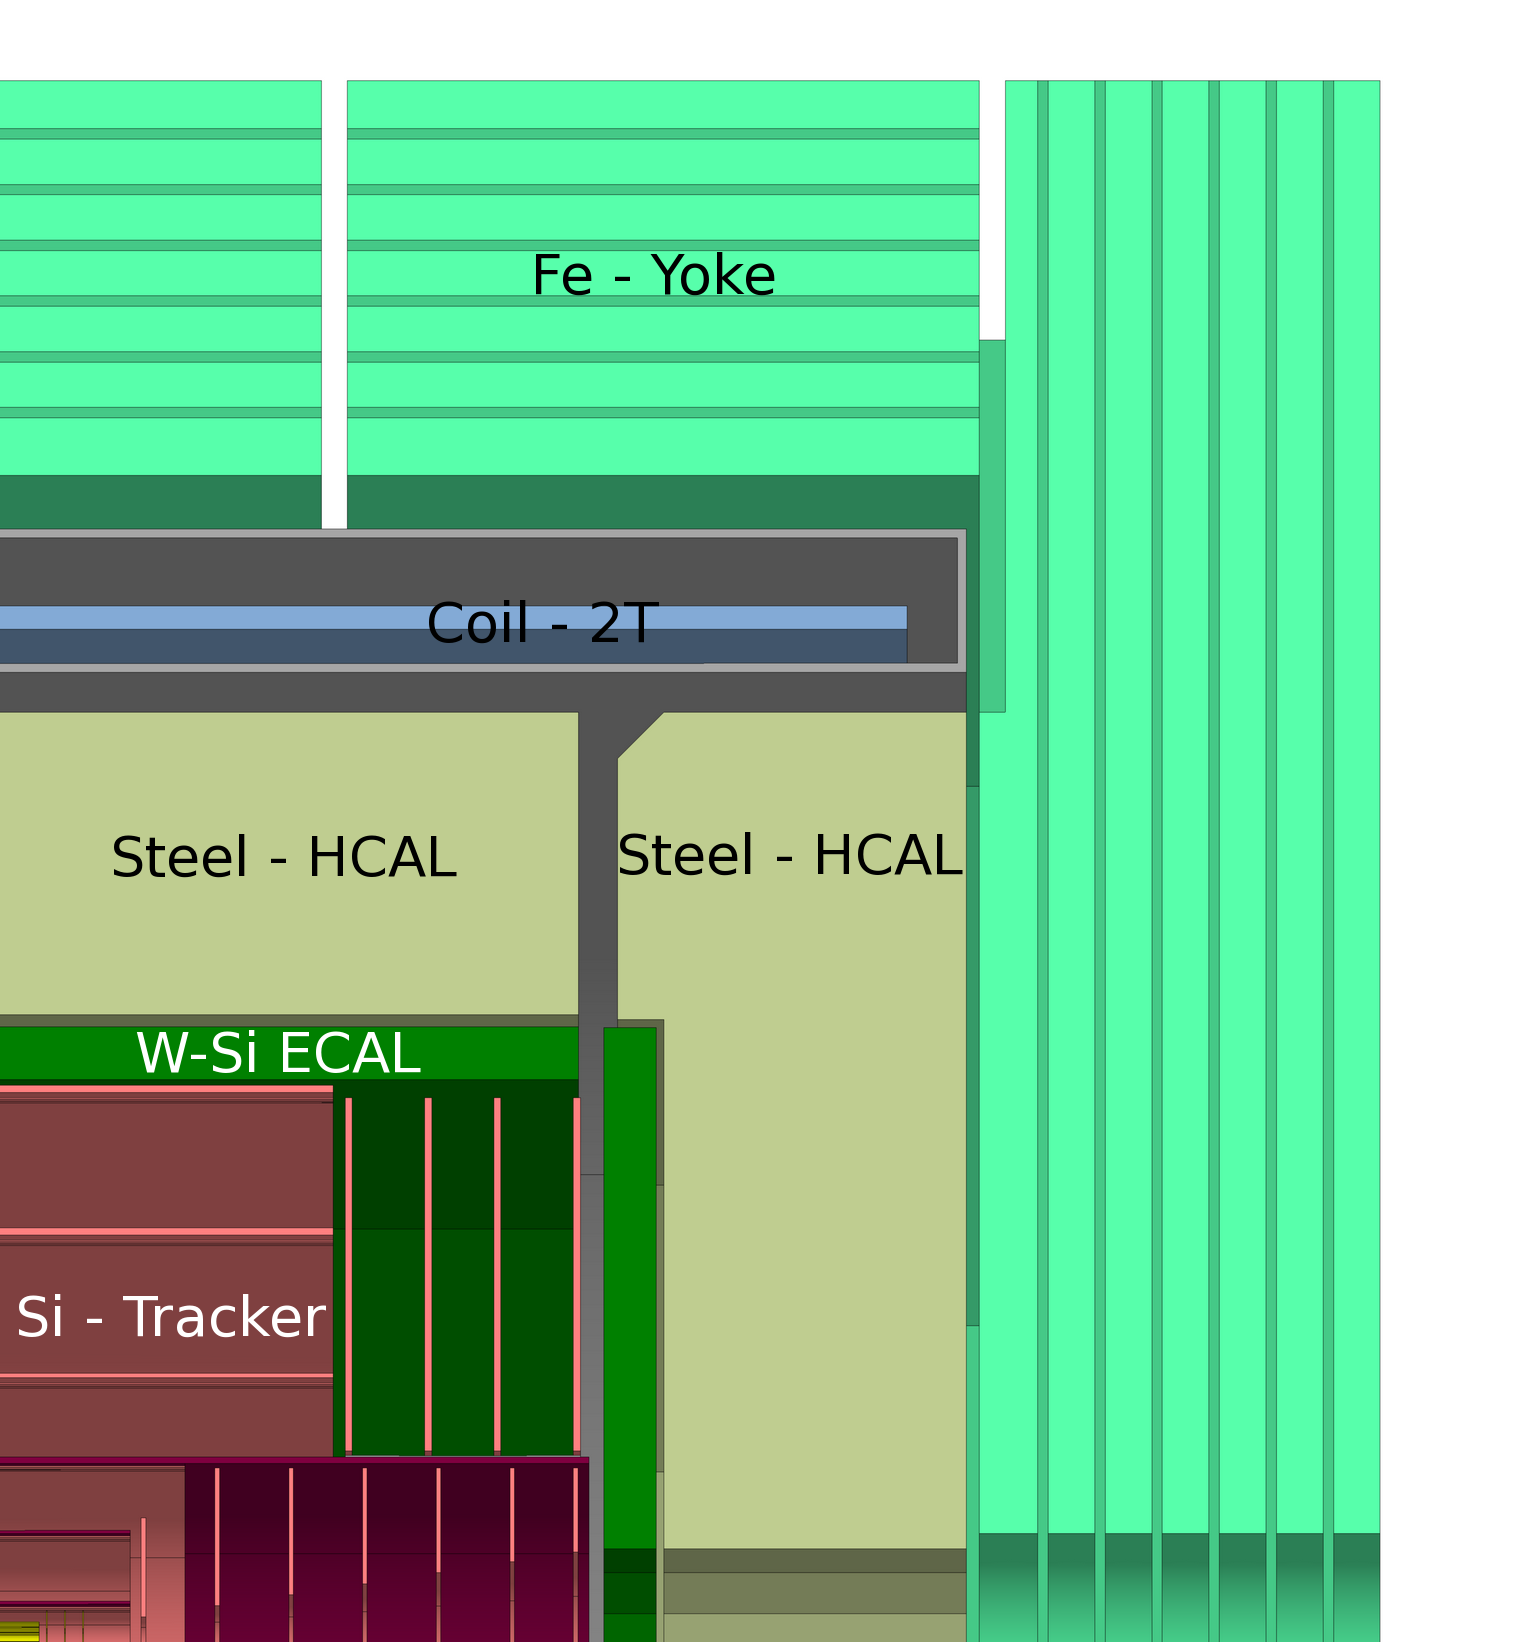
\includegraphics[width=7.8cm]{../CEPC_workshop/FCCeePictsFromKonrad/CLIC_FCC_Top_QuarterView_withLabes.png}};
% 
% \node  at (\xRefPosOne,\yRefPosOne+2.8) (box){%
% \myCenterBox{\small CLD model}
% }; 
%     
%     \draw[black, thick, ->] (-0.8,-4.76)--(-0.8,3.7) node[pos=0.95, right]{\small R [m]};
%     \draw[black, thick, ->] (-0.8,-4.76)--(6.5,-4.76) node[pos=0.95, below]{\tiny Z [m]};
%     
%   \node[inner sep=0pt] (tmp) at (\xRefPosOne-3.05,\yRefPosOne-4.9)
%     {2.3};   
%   \node[inner sep=0pt] (tmp) at (\xRefPosOne-1.14,\yRefPosOne-4.9)
%     {3.7};  
    
%     \node [PixelBox] at (\xRefPosOne+3.7,\yRefPosOne-4) (box){%
%   \begin{minipage}{0.43\textwidth}
%     Detector design inspired by detectors for CLIC and ILC and optimized for FCC-ee conditions
%   \end{minipage}
% };

\node  at (\xRefPosOne+3.5,\yRefPosOne-0.5) (box){%
    \begin{minipage}{0.5\textwidth}

  \begin{itemize}
      \item TODO [previous slide] - superimpose CLICdet tracker + ECAL and show for each detector direction of ECAL crack with angles written
      \item TODO Comparison of material udgets for tracker; explain that we need more material in CLD for coolings
  \end{itemize}

    \end{minipage}
};


% \node [PixelBox] at (\xRefPosOne+3.7,\yRefPosOne-4) (box){%
%   \begin{minipage}{0.43\textwidth}
%     Detector design inspired by detectors for CLIC and ILC and optimized for FCC-ee conditions
%   \end{minipage}
% };

%% HELPER draw advanced helping grid with axises:
% \draw(-0.5,-4) to[grid with coordinates] (11.5,4);
\end{tikzpicture}

 
\end{frame}
%*****************************************************************************


%*****************************************************************************
% \bgroup
% \setbeamercolor{background canvas}{bg=white}
\begin{frame}{}

    \begin{tikzpicture}[overlay]

    %% HELPER draw advanced helping grid with axises:
%     \draw (0,-5) to[grid with coordinates] (11,3);

    \node[right] (textNode) at (3.5,0) {
      {\large \bf Software Compensation}
    };
    

    \end{tikzpicture}

\end{frame}
% \egroup
%*****************************************************************************

%*****************************************************************************
\begin{frame}{\large \large Software Compensation}
\renewcommand{\yRefPosOne}{0}
\renewcommand{\xRefPosOne}{5.3}
\renewcommand{\xRefIncrementOne}{5.5}

 \begin{tikzpicture}[overlay]
 
%   \node[inner sep=0pt] (tmp) at (\xRefPosOne,\yRefPosOne+0.5)
%     {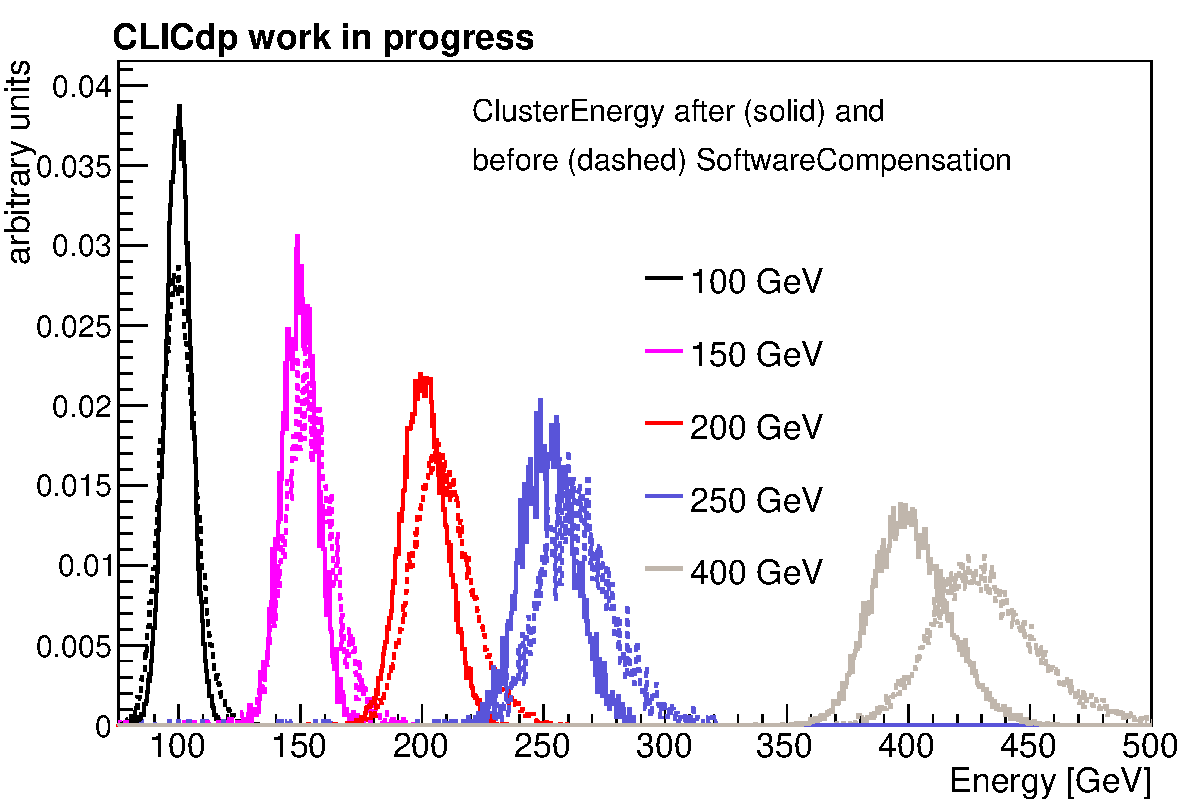
\includegraphics[width=8cm]{Matthias/ClosurePlotOfHighEnergyRangeNeutrons.pdf}};

 
 \node  at (\xRefPosOne,\yRefPosOne-3.5) (box){%
    \begin{minipage}{\textwidth}

  \begin{itemize}
   \item ???
  \end{itemize}

    \end{minipage}
};

\end{tikzpicture}
 
\end{frame}
%*****************************************************************************


%*****************************************************************************
\begin{frame}{\large \large Software Compensation at CLIC}
\renewcommand{\yRefPosOne}{0}
\renewcommand{\xRefPosOne}{5.3}
\renewcommand{\xRefIncrementOne}{5.5}

 \begin{tikzpicture}[overlay]
 
  \node[inner sep=0pt] (tmp) at (\xRefPosOne,\yRefPosOne+0.5)
    {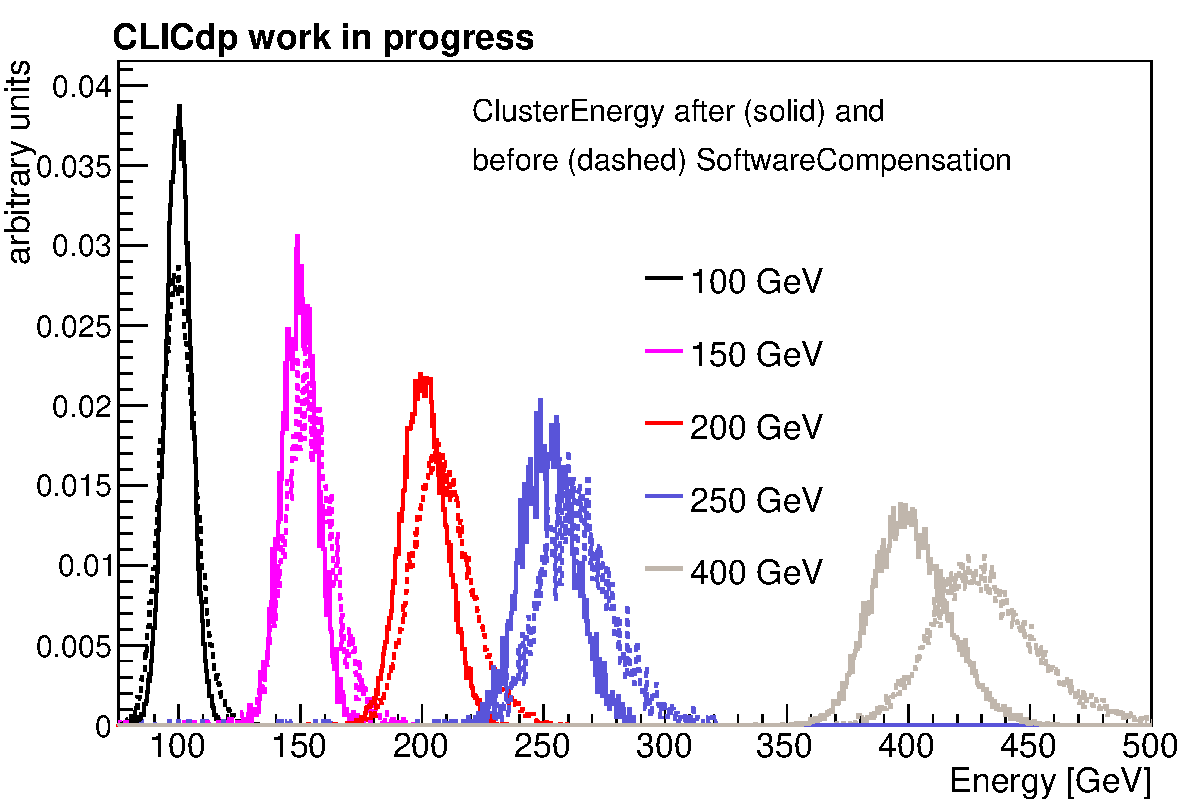
\includegraphics[width=8cm]{Matthias/ClosurePlotOfHighEnergyRangeNeutrons.pdf}};

 
 \node  at (\xRefPosOne,\yRefPosOne-3.5) (box){%
    \begin{minipage}{\textwidth}

  \begin{itemize}
   \item Software compensation weights derived from MC using neutron and $K_L^0$ events
   \item Mean and resolution after software compensation largely improved
   \item Software compensation corrects for nonlinear response of hadrons on the fly
  \end{itemize}

    \end{minipage}
};

\end{tikzpicture}
 
\end{frame}
%*****************************************************************************

%*****************************************************************************
\begin{frame}{\large \large Jet energy resolution at CLIC with dijet events}

\renewcommand{\yRefPosOne}{-0.5}
\renewcommand{\xRefPosOne}{5.3}
\renewcommand{\xRefIncrementOne}{5.5}
\begin{tikzpicture}[overlay]

 \node[inner sep=0pt] (tmp) at (\xRefPosOne-3,\yRefPosOne+1.2)
    {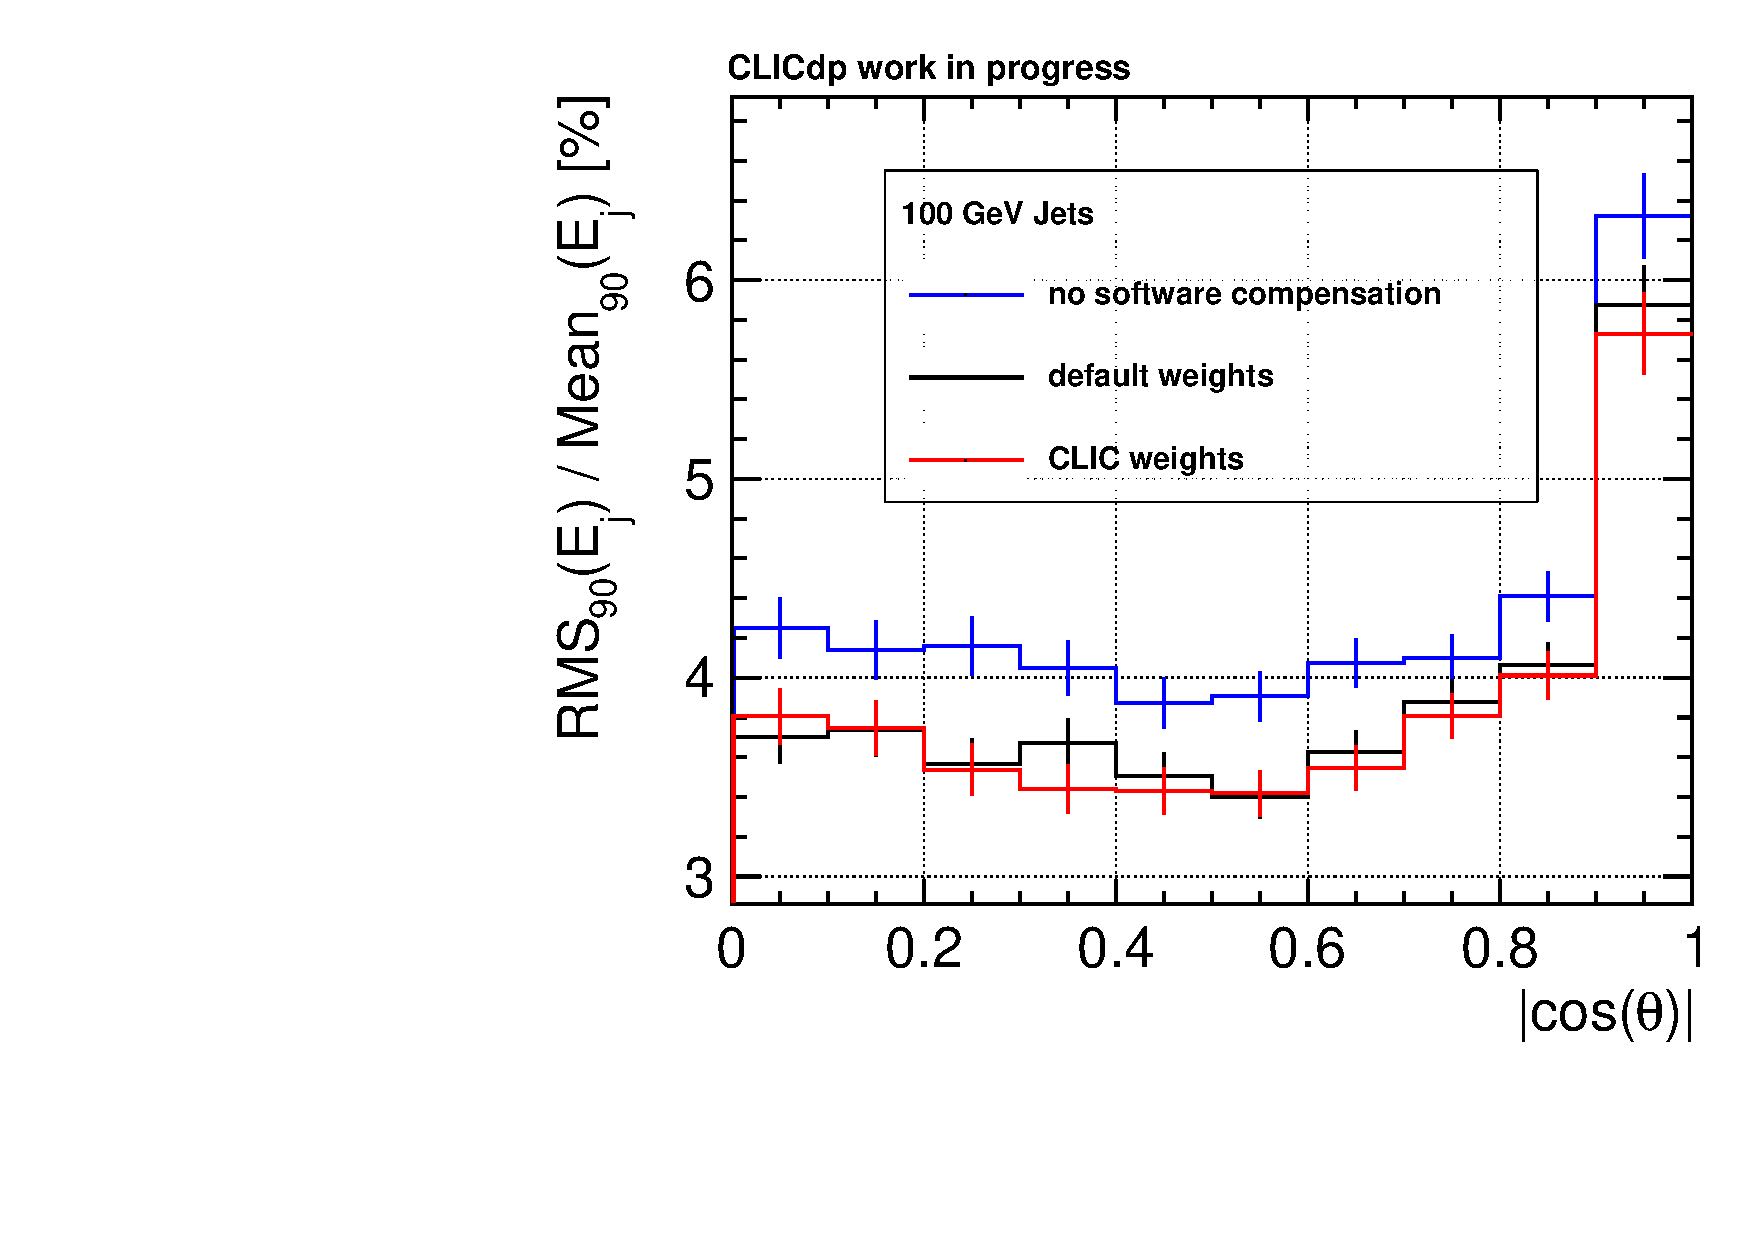
\includegraphics[width=5.5cm]{Matthias/Zuds200_RMS90_vs_cosTheta_Quark_100GeV_Jets_noSWC_ILDWeights_CLICWeights.pdf}};
    
 \node[inner sep=0pt] (tmp) at (\xRefPosOne+3,\yRefPosOne+1.25)
    {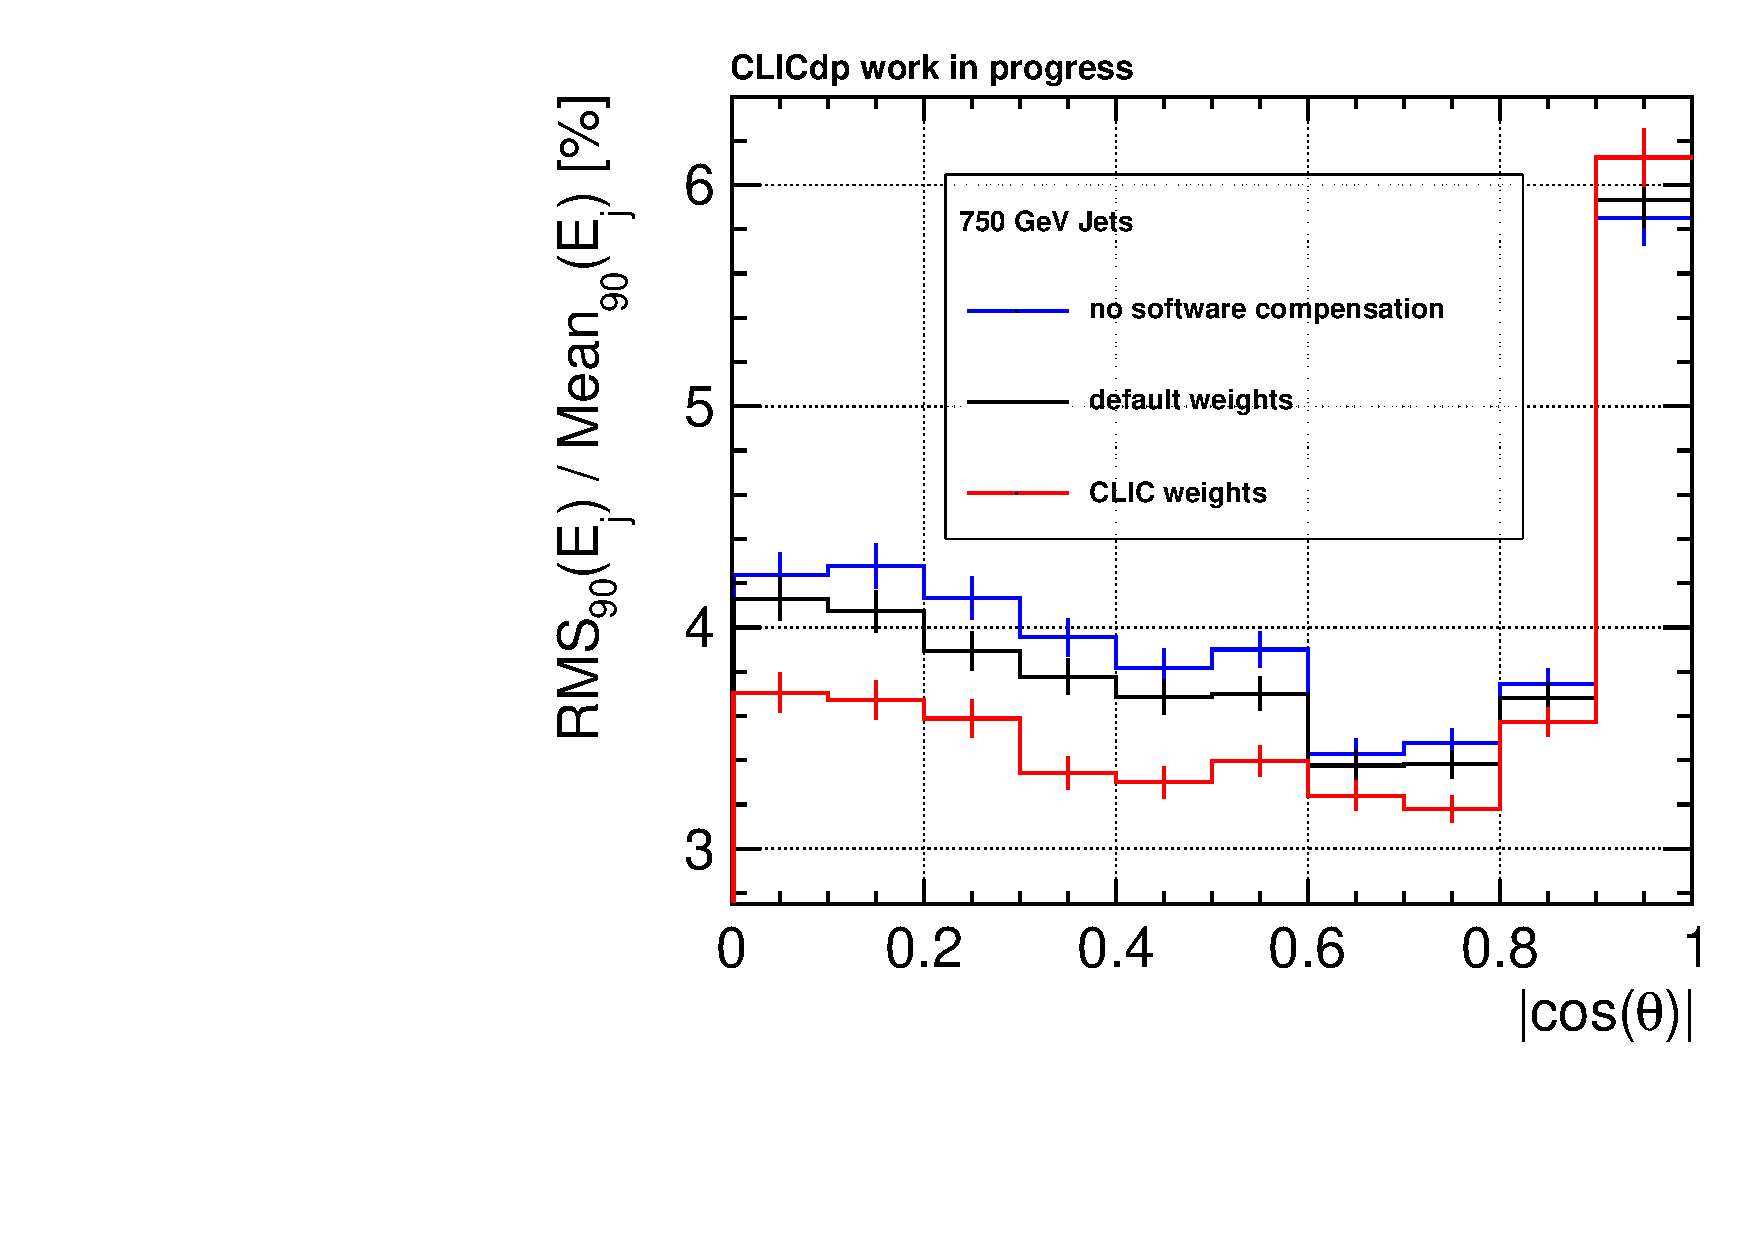
\includegraphics[width=5.5cm]{Matthias/Zuds1500_RMS90_vs_cosTheta_Quark_750GeV_Jets_noSWC_ILDWeights_CLICWeights.pdf}};
    
%  \node[inner sep=0pt] (tmp) at (\xRefPosOne-1.6,\yRefPosOne+0.1)
%     {\tiny WORK IN PROGRESS};
%  \node[inner sep=0pt] (tmp) at (\xRefPosOne+4.5,\yRefPosOne-0.1)
%     {\tiny WORK IN PROGRESS};
    
\node  at (\xRefPosOne-3.2,\yRefPosOne+2.8) (box){%
\myCenterBox{\small 100 GeV jets}
}; 

\node  at (\xRefPosOne+3.05,\yRefPosOne+2.8) (box){%
\myCenterBox{\small 750 GeV jets}
}; 



\node  at (\xRefPosOne,\yRefPosOne-2.8) (box){%
\begin{minipage}{\textwidth}
  \begin{itemize}
   \item applying software compensation always improves jet energy resolution
   \item comparable performance of CLIC tuned weight at low jet energies (left plot)
   \item significant improvement at high jet energies (right plot)
  \end{itemize}
\end{minipage}
};


% % HELPER draw advanced helping grid with axises:
% \draw(-0.5,-4) to[grid with coordinates] (11.5,4);
\end{tikzpicture}
 
\end{frame}
%*****************************************************************************

%*****************************************************************************
\begin{frame}{\large \large Jet energy resolution at CLIC with dijet events}

\renewcommand{\yRefPosOne}{-0.5}
\renewcommand{\xRefPosOne}{5.3}
\renewcommand{\xRefIncrementOne}{5.5}
\begin{tikzpicture}[overlay]

 \node[inner sep=0pt] (tmp) at (\xRefPosOne-3,\yRefPosOne+1.2)
    {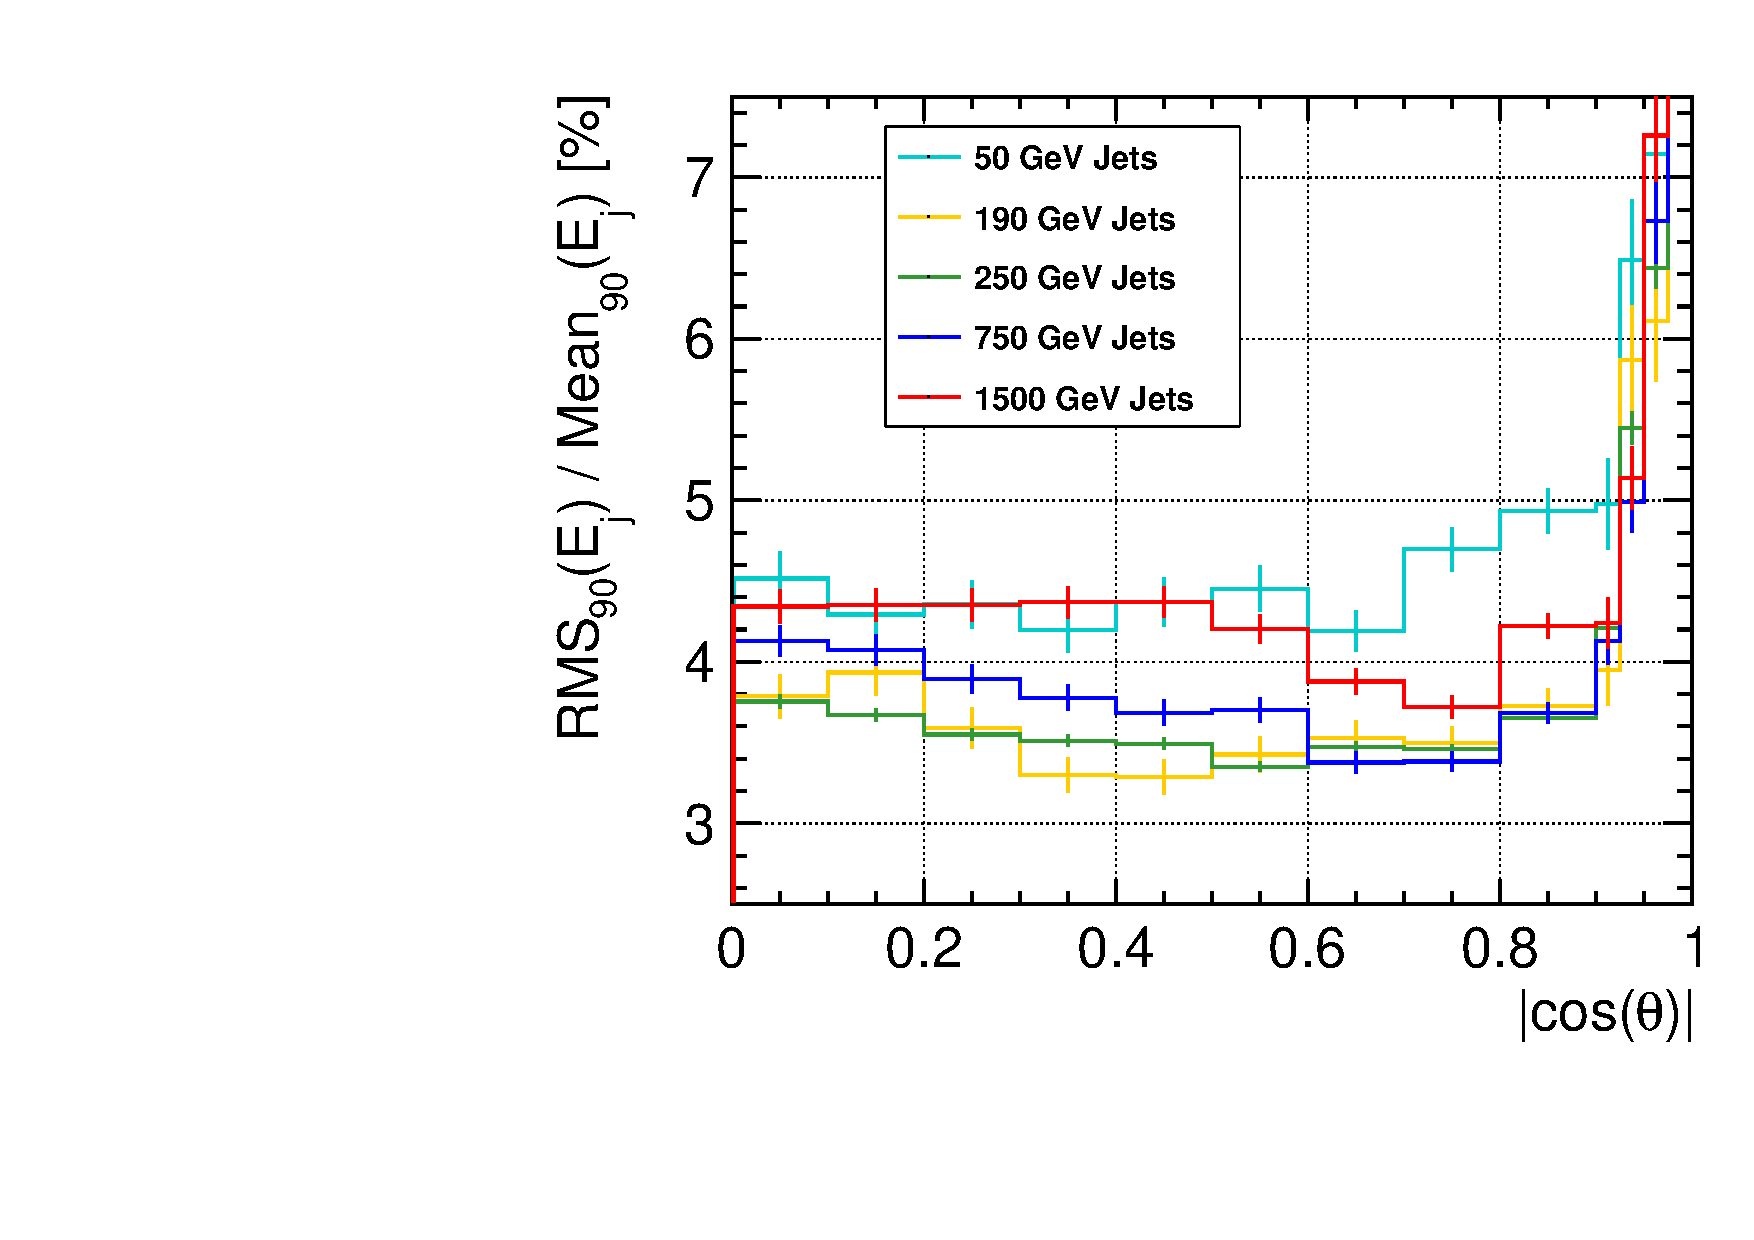
\includegraphics[width=5.5cm]{Matthias/JER_Summary_ILD_Red.pdf}};
    
 \node[inner sep=0pt] (tmp) at (\xRefPosOne+3,\yRefPosOne+1.25)
    {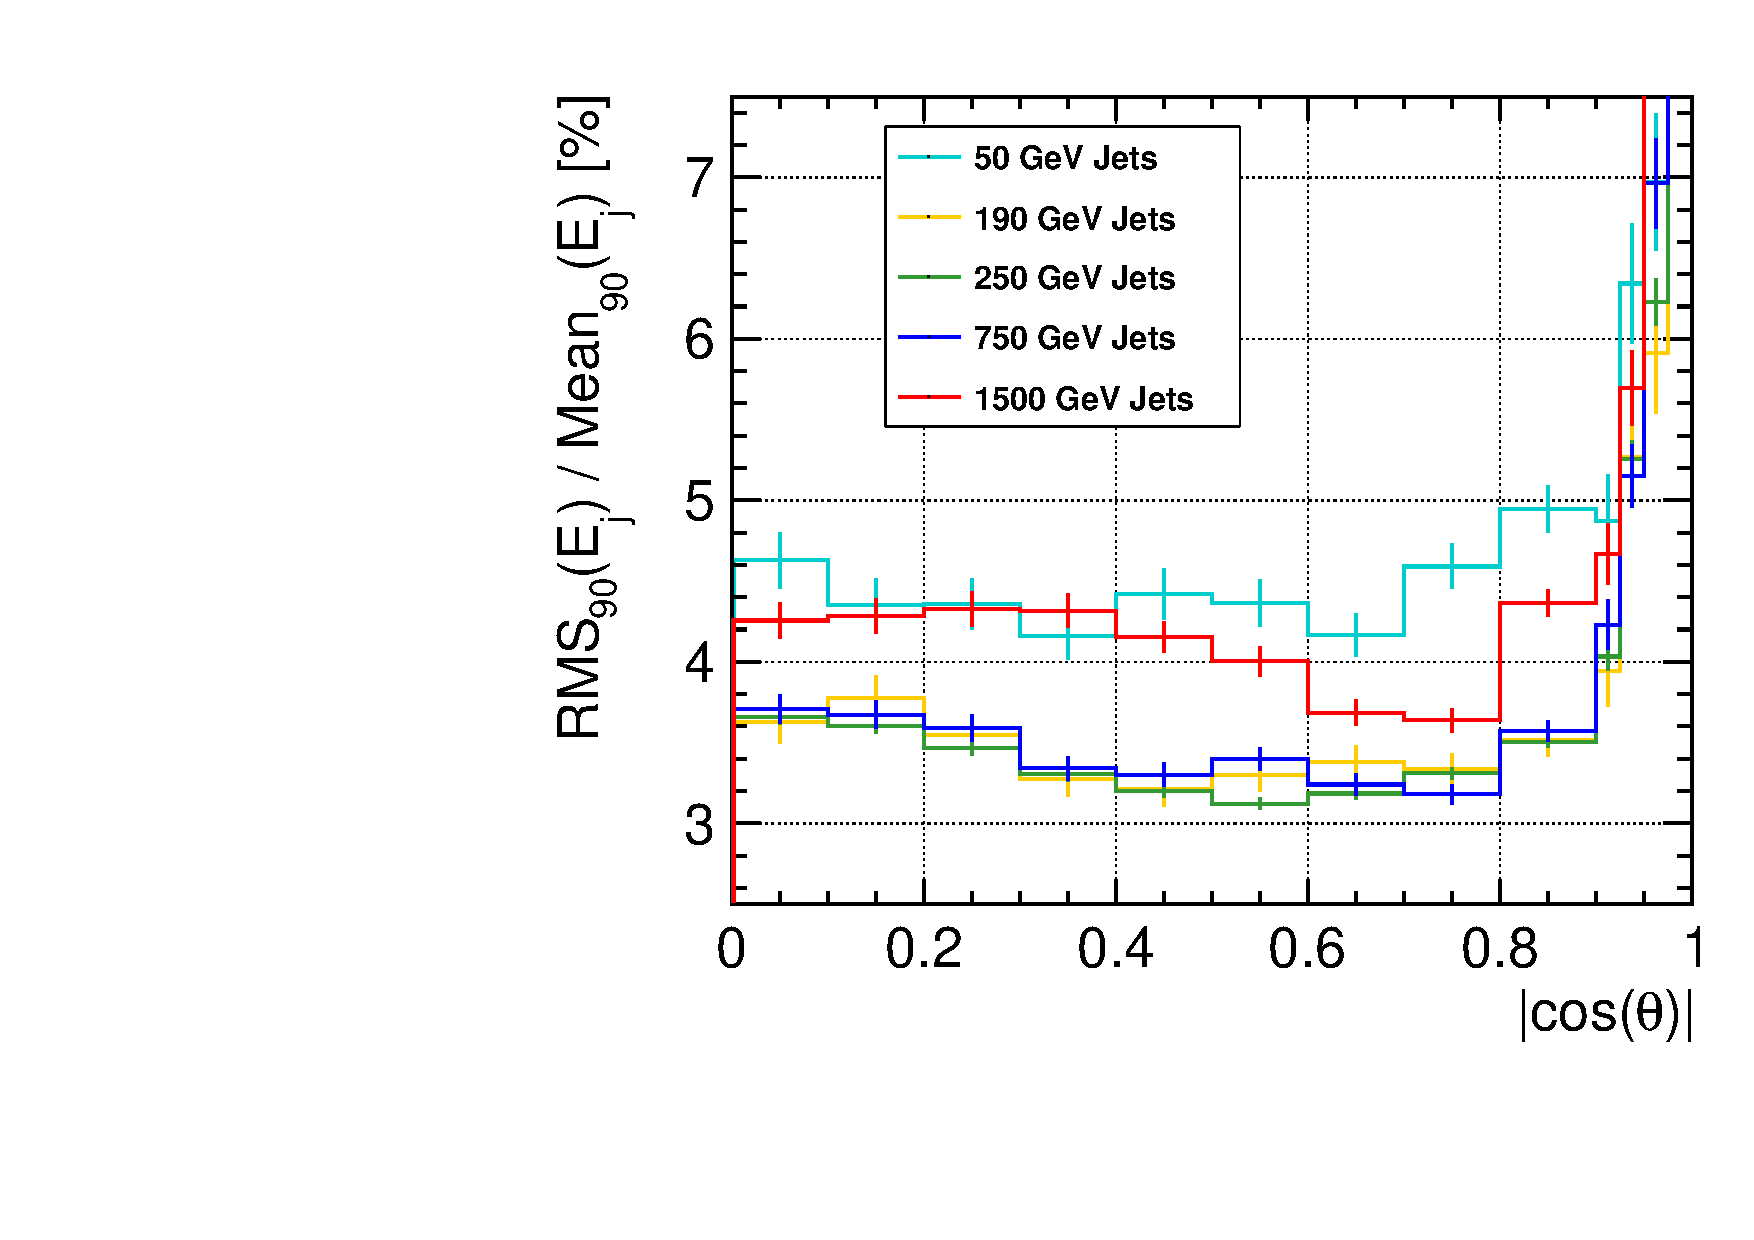
\includegraphics[width=5.5cm]{Matthias/JER_Summary_CLIC_n_K0L_Red.pdf}};

\node  at (\xRefPosOne-1.7,\yRefPosOne+3.2) (box){%
\myCenterBox{\small default weights}
}; 

\node  at (\xRefPosOne+4.45,\yRefPosOne+3.2) (box){%
\myCenterBox{\small CLIC weights}
}; 

 \node[inner sep=0pt] (tmp) at (\xRefPosOne-3.79,\yRefPosOne+3.42)
    {
\includegraphics[width=2.0cm]{Matthias/clicdp_work_in_progress.pdf}};

 \node[inner sep=0pt] (tmp) at (\xRefPosOne+2.21,\yRefPosOne+3.42)
    {
\includegraphics[width=2.0cm]{Matthias/clicdp_work_in_progress.pdf}};

\node  at (\xRefPosOne,\yRefPosOne-2.8) (box){%
\begin{minipage}{\textwidth}
  \begin{itemize}
   \item Comparable performance for jets up to 190 GeV
   \item Improvement of jet energy resolutions by around 10$\%$ for larger jet energies 
   \item Achive jet energy resolution between 3.1 $\%$ and 4.5 $\%$ with CLIC tuned weights 
  \end{itemize}
\end{minipage}
};


% % HELPER draw advanced helping grid with axises:
% \draw(-0.5,-4) to[grid with coordinates] (11.5,4);
\end{tikzpicture}
 
\end{frame}
%*****************************************************************************


%*****************************************************************************
\begin{frame}{\large \large Summary}
 
 \renewcommand{\yRefPosOne}{0}
\renewcommand{\xRefPosOne}{5.3}
\renewcommand{\xRefIncrementOne}{5.5}
\begin{tikzpicture}[overlay]

      
\node  at (\xRefPosOne,\yRefPosOne) (box){%
  \begin{minipage}{0.99\textwidth}
 \begin{itemize}
  \item ???
%   \item The second detector design which consist of drift chamber and dual readout calorimeter 
  

%   \item Performance study based on the full simulation demonstrated impressive detector performance 
%   \item TODO to mention IDEA detector concept???
  
    \end{itemize}
  \end{minipage}
};

\node[right] (textNode) at (3,-3) {
      { \large \bf Thank you for attention! }
    };

\end{tikzpicture}
  
\end{frame}
%*****************************************************************************

\backupbegin

%------------------------------------------------
\begin{frame}
\frametitle{BACKUP} 
 
\end{frame}

\backupend

\end{document}

